% vim: spelllang=en
\section{Theory}\label{theory}

A diode laser is a cheap and tiny alternative to dye-lasers, therefore it is often used at student
labs.
In this report the absorption spectrum of rubidium (Rb) is studied, to gain knowledge of using
a diode laser.

\subsection{Introduction}\label{introduction}

A laser consists of three components:

\begin{enumerate}
  \item pump source
  \item optical medium
  \item cavity / resonator
\end{enumerate}

When an excited electron relaxes, it is able to emit a photon.
To excite electrons of the optical medium into states of higher energy, a pump source is used.
This could be another laser, biological effects, or, as it is in this case, a current.

Now with the electrons of the optical medium in the excited states, there are four possible
effects, grouped in two categories.
The first group is the non-radiative relaxation, where the energy of the electrons is transferred
to the medium lattice, the so-called phonons.
The second group is radiative relaxation, with spontaneous and induced emission.
Spontaneous emission is the effect, where an electron spontaneously relaxes into a lower energy
state, emitting a photon.

The most important effect for lasers is induced emission.
The energy of an incoming photon induces the emission of another photon.
The two photons are coherent, which means they have the same phase.

See figure~\ref{fig:two_niveau_laser} for a visualisation of these radiative effects.
\begin{figure}[ht]
  \centering
  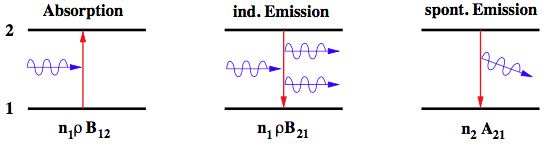
\includegraphics[width=0.8\linewidth]{content/zweiniveausystem.png}
  \caption{Visualisation of radiative effects with two energy states\cite{anleitung_hene}.}%
  \label{fig:two_niveau_laser}
\end{figure}

The cavity is used as a resonator (see figure~\ref{fig:resonator}) in which the photons
travel many times through the optical medium to induce emission of coherent photons.

\begin{figure}[ht]
  \centering
  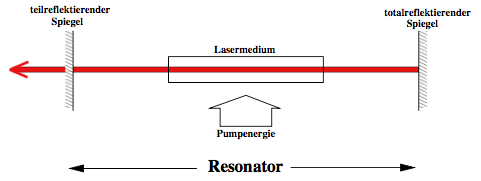
\includegraphics[width=0.8\linewidth]{content/resonator.png}
  \caption{Schematic view of a resonator with one semipermeable mirror and a totally reflective
  mirror\cite{anleitung_hene}.}%
  \label{fig:resonator}
\end{figure}

The difference in frequencies of a laser is calculated as follows:
\begin{align}\label{eq:free_spectral_range}
  \Delta \nu &= \frac{c}{2Ln},
\end{align}
with $n$ being the refraction index of the optical medium, $L$ the resonator length
and $c$ the speed of light.
As seen clearly, by changing the length of the resonator a range of frequency is scanned.


\subsection{Diodes}\label{diodes}

A diode is a p-n-doped semiconductor.
In the n-plane electrons are added, that the plane has negative charge.
On the other hand ions are added to the p-plane so that it has positive charge.
These so-called electron-hole pairs build an electric field between the planes.
If current is applied either the current flows through or it is blocked due to the depleted region
between the planes (in the middle of the \enquote{space charge region},
see figure~\ref{fig:depletion_region}).
\begin{figure}[ht]
  \centering
  \includegraphics[width=0.8\linewidth]{build/pn_diode.png}
  \caption{Schematic view of a p-n-diode\cite{pn_diode_wiki}.}%
  \label{fig:depletion_region}
\end{figure}

A light emitting diode (LED) emits light when activated.
The recombination of electron-hole pairs releases energy in form of photons.

\subsection{Three state laser}\label{three-state-laser}

According to the Boltzmann distribution the ground state is always most populated in thermal
equilibrium.
At least three states are needed for a laser to lase: The pump source excites the electrons from
the ground state up to the highest exited state.
The lifetime \(\tau_1\) of electrons in this energy state is very short, the electrons relax
spontaneously two the second but lower excited state, where they have a much longer lifetime
\(\tau_2 \gg \tau_1\).
In the second excited state electrons can be kicked out by incoming photons, emitting coherent
radiation (induced emission).
For an example the energy states of a four state laser are shown in
figure~\ref{fig:four_state_laser}.
\begin{figure}[ht]
  \centering
  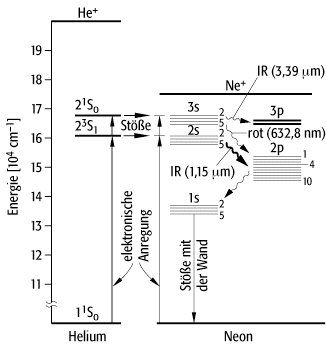
\includegraphics[width=0.6\linewidth]{content/uebergaenge.jpg}
  \caption{Energy states and transitions of a four state helium neon laser\cite{anleitung_hene}.}%
  \label{fig:four_state_laser}
\end{figure}

\subsection{Operation principle of a diode laser}\label{sub:diode-laser}
\begin{figure}[ht]
  \centering
  \includegraphics[width=0.8\linewidth]{build/cutawayview.pdf}
  \caption{Cut-away view of a typical laser diode can\cite{anleitung}.}%
  \label{fig:cutawayview}
\end{figure}
\begin{figure}[ht]
  \centering
  \includegraphics[width=0.8\linewidth]{build/laser_diode_chip.pdf}
  \caption{Schematic view of a laser diode chip\cite{anleitung}.}%
  \label{fig:laser_diode_chip}
\end{figure}
\subsection{Tuning of the diode laser}\label{tuning-of-the-diode-laser}

There are many options to alter the lasing function of the diode used in this experiment.
Each option alters different attributes of the laser, which will be elaborated in the following.
As a summary their effects are displayed in figure~\ref{fig:lasertuning}.
\begin{figure}[ht]
  \centering
  \includegraphics[width=0.8\linewidth]{build/lasertuning.pdf}
  \caption{The net gain of the laser in relation to the lasing wavelength, sorted by the different
  tuning options\cite{anleitung}.}%
  \label{fig:lasertuning}
\end{figure}

\subsubsection{Medium gain}\label{medium-gain}
The medium gain depends on the size of the depleted region, called band gap.
It is visualized as the broad peak in figure~\ref{fig:lasertuning}.
Since the location of the band gap depends mainly on the temperature of the laser,
it is set so that the resulting wavelength is about \SI{780}{\nano\meter},
the resonance line of rubidium,
which means a laser temperature of \SI{50}{\celsius}.

\subsubsection{Internal cavity}\label{internal-cavity}
The diode forms an optical cavity, which translates to a periodic net gain function
that is dependent on frequency.
This is called \enquote{free spectral range} and is defined by
equation~\eqref{eq:free_spectral_range}.
In this diode the refraction index is $n = \num{3.6}$\cite{anleitung}.
This yields $\Delta \nu = \SI{60}{\giga\hertz}$ and $\Delta \lambda = \SI{0.122}{\nano\meter}$.
The frequency shifts with changes in the laser temperature at \SI{0.05}{\nano\meter\per\celsius},
which means that with a higher laser current the wavelength of the diode laser changes accordingly.
The laser current additionally changes the wavelength in another way:
The altered carrier concentration in the active region modulates the path length of the diode,
and thus the wavelength of the laser.

As seen the temperature changes shift the wavelengths and is itself changed by the laser current.
The wavelength shift rates are differently in both explained effects, which creates \enquote{mode
hops}, sudden changes in the operating mode of the laser.

The sensitivity to optical feedback is utilized to simplify the tuning of the laser.

\subsubsection{Grating feedback}\label{grating-feedback}
The dispersed light coming from a grating has a narrow bandwidth.
A rotatable diffraction grating is used to point the first Bragg reflection
\begin{align}
  n \lambda &= 2 d \sin\!{\vartheta}
\end{align}
back into the active layer of the diode laser.
This is called \enquote{Littrow configuration}.
The feedback is used to stabilize the frequencies of the laser.

\subsubsection{External cavity}\label{external-cavity}
The external cavity ranges from the reflective back of the diode to the grating.
Due to the much higher cavity length $\Delta \nu \approx \SI{10}{\giga\hertz}$.
The position of the grating is either changed by hand or with the piezo-electric transducer (see
section~\ref{sub:piezo-element}).

To operate the laser at the predetermined wavelength of rubidium absorption of
$\lambda_0 = \SI{780}{\nano\meter}$ the net gains of all four components should
peak at $\lambda_0$ as illustrated in figure~\ref{fig:lasertuning}.

A scan of various settings and corresponding gains and possible mode hops is
displayed in figure~\ref{fig:lasertuning_modehops}.
\begin{figure}[ht]
  \centering
  \includegraphics[width=0.8\linewidth]{build/lasertuning_modehops.pdf}
  \caption{Series of graphs showing different settings of the  components of
    the laser tuning and their respective mode hops\cite{anleitung}.}%
  \label{fig:lasertuning_modehops}
\end{figure}

\subsection{Piezo element}\label{sub:piezo-element}
Piezoelectric charge accumulates in certain solid materials in response to mechanical stress.
This effect can be used backwards, as piezo-crystals change their dimensions with applied voltage.

\subsection{Experiment setup}\label{experiment-setup}
Due to the strongly diverging light a collimating lens is used directly behind the output facet of
the diode laser.
See figure~\ref{fig:experiment-setup} for a schematic view of the laser component of the
experiment.

\begin{figure}[ht]
  \centering
  \includegraphics[width=0.8\linewidth]{build/basicconfiguration.pdf}
  \caption{Schematic view of the laser in the experiment\cite{anleitung}.}%
  \label{fig:experiment-setup}
\end{figure}

The laser contains two knobs, a head knob and a side knob.
These are used to tilt the diffraction grating in two ways.
The head knob rotates the vertical grating angle,
which should be set so that the diffracted light shines straight through the active layer of the
diode.
The side knobs rotates the grating horizontal, i.e.\ it changes the frequency of the diffracted
light which in turn changes the grating feedback in the diode.
